% SPDX-License-Identifier: BSD-2-Clause
%
% Copyright (C) 2026 embedded brains GmbH & Co. KG
%
% Redistribution and use in source and binary forms, with or without
% modification, are permitted provided that the following conditions
% are met:
% 1. Redistributions of source code must retain the above copyright
%    notice, this list of conditions and the following disclaimer.
% 2. Redistributions in binary form must reproduce the above copyright
%    notice, this list of conditions and the following disclaimer in the
%    documentation and/or other materials provided with the distribution.
%
% THIS SOFTWARE IS PROVIDED BY THE COPYRIGHT HOLDERS AND CONTRIBUTORS "AS IS"
% AND ANY EXPRESS OR IMPLIED WARRANTIES, INCLUDING, BUT NOT LIMITED TO, THE
% IMPLIED WARRANTIES OF MERCHANTABILITY AND FITNESS FOR A PARTICULAR PURPOSE
% ARE DISCLAIMED. IN NO EVENT SHALL THE COPYRIGHT OWNER OR CONTRIBUTORS BE
% LIABLE FOR ANY DIRECT, INDIRECT, INCIDENTAL, SPECIAL, EXEMPLARY, OR
% CONSEQUENTIAL DAMAGES (INCLUDING, BUT NOT LIMITED TO, PROCUREMENT OF
% SUBSTITUTE GOODS OR SERVICES; LOSS OF USE, DATA, OR PROFITS; OR BUSINESS
% INTERRUPTION) HOWEVER CAUSED AND ON ANY THEORY OF LIABILITY, WHETHER IN
% CONTRACT, STRICT LIABILITY, OR TORT (INCLUDING NEGLIGENCE OR OTHERWISE)
% ARISING IN ANY WAY OUT OF THE USE OF THIS SOFTWARE, EVEN IF ADVISED OF THE
% POSSIBILITY OF SUCH DAMAGE.

\documentclass[tikz,border=4pt]{standalone}
\usepackage[T1]{fontenc}
\usepackage[scaled]{helvet}
\renewcommand{\familydefault}{\sfdefault}
\usetikzlibrary{arrows.meta,positioning,fit,backgrounds,shapes.geometric}
\definecolor{ebblue}{HTML}{1F4E79}
\definecolor{boxfill}{HTML}{EAF1F8}
\definecolor{codefill}{HTML}{FFF4E0}
\definecolor{codeline}{HTML}{9C6500}
\definecolor{groupfill}{HTML}{F5F5F5}
\definecolor{flow}{HTML}{404040}
\newcommand{\code}[1]{{\ttfamily\scriptsize #1}}
\begin{document}
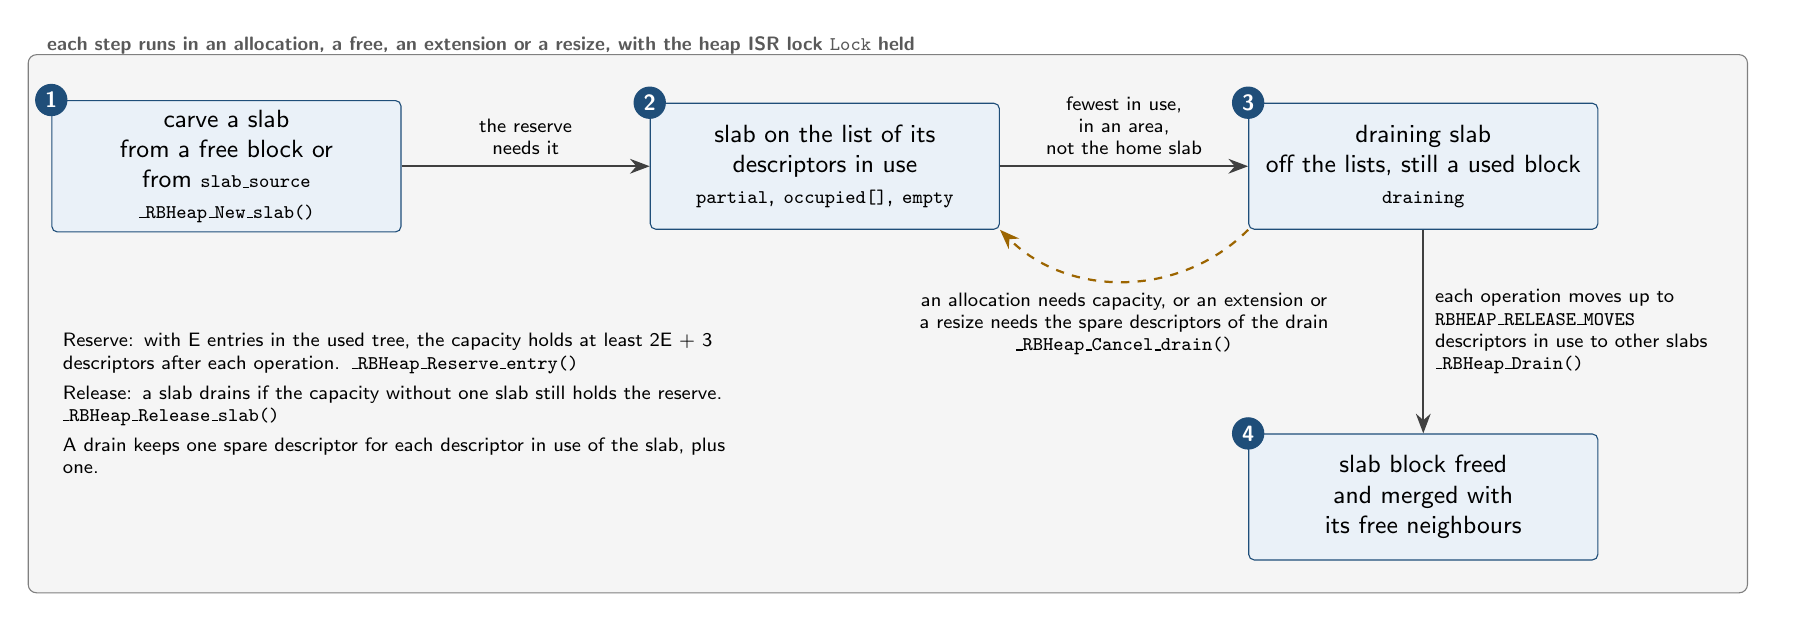
\begin{tikzpicture}[
    font=\small,
    state/.style={draw=ebblue, fill=boxfill, rounded corners=2pt,
      minimum width=44mm, minimum height=16mm, align=center, text width=42mm},
    num/.style={circle, draw=ebblue, fill=ebblue, text=white,
      font=\footnotesize\bfseries, inner sep=1.5pt},
    trans/.style={-{Stealth[length=2.5mm]}, thick, draw=flow},
    cancel/.style={-{Stealth[length=2.5mm]}, thick, dashed, draw=codeline},
    lbl/.style={font=\scriptsize, align=center, inner sep=1pt,
      text width=28mm},
    lockframe/.style={fill=groupfill, draw=gray, rounded corners=3pt}]
  \node[state] (carve) at (0,0) {carve a slab\\from a free block or\\from \code{slab\_source}\\\code{\_RBHeap\_New\_slab()}};
  \node[state] (list) at (7.6,0) {slab on the list of its\\descriptors in use\\\code{partial}, \code{occupied[]}, \code{empty}};
  \node[state] (drain) at (15.2,0) {draining slab\\off the lists, still a used block\\\code{draining}};
  \node[state] (freed) at (15.2,-4.2) {slab block freed\\and merged with\\its free neighbours};
  \node[num] at (carve.north west) {1};
  \node[num] at (list.north west) {2};
  \node[num] at (drain.north west) {3};
  \node[num] at (freed.north west) {4};
  \draw[trans] (carve) -- node[lbl, above=1mm] {the reserve\\needs it} (list);
  \draw[trans] (list) -- node[lbl, above=1mm] {fewest in use,\\in an area,\\not the home slab} (drain);
  \draw[trans] (drain) -- node[lbl, right=1mm, text width=44mm, align=left]
    {each operation moves up to\\\code{RBHEAP\_RELEASE\_MOVES}\\descriptors in use to other slabs\\\code{\_RBHeap\_Drain()}} (freed);
  \draw[cancel] (drain.south west) to[out=225, in=315] node[lbl, below=1mm, text width=60mm]
    {an allocation needs capacity, or an extension or a resize needs the spare
     descriptors of the drain\\\code{\_RBHeap\_Cancel\_drain()}} (list.south east);
  \node[font=\scriptsize, align=left, anchor=north west, text width=85mm] at (-2.2,-2.0)
    {Reserve: with E entries in the used tree, the capacity holds at least 2E + 3
     descriptors after each operation.  \code{\_RBHeap\_Reserve\_entry()}\\[1mm]
     Release: a slab drains if the capacity without one slab still holds the
     reserve.  \code{\_RBHeap\_Release\_slab()}
    \\[1mm]
     A drain keeps one spare descriptor for each descriptor in use of the slab,
     plus one.};
  \begin{scope}[on background layer]
    \node[lockframe, fit={(-2.4,1.3) (19.2,-5.3)}] {};
  \end{scope}
  \node[font=\scriptsize\bfseries, text=gray!70!black, anchor=south west] at (-2.4,1.3) {each step runs in an allocation, a free, an extension or a resize, with the heap ISR lock \code{Lock} held};
\end{tikzpicture}
\end{document}
